% Source - https://tex.stackexchange.com/a
% Posted by Martin Scharrer, modified by community. See post 'Timeline' for change history
% Retrieved 2026-01-20, License - CC BY-SA 3.0
\documentclass[tikz,convert={outfile=\jobname.svg}]{standalone}
\usetikzlibrary{calc, arrows.meta, positioning, shapes.symbols, shapes.geometric}

\tikzset{
  vec/box/.style={draw, rounded corners=2pt, thick, align=center, inner sep=4pt},
  vec/small/.style={draw, rounded corners=2pt, thick, align=center, inner sep=2pt, font=\small},
  vec/arrow/.style={-Latex, thick},
  vec/darrow/.style={<->, Latex-Latex, thick},
  vec/dot/.style={circle, fill, inner sep=1.3pt},
  vec/title/.style={font=\small\bfseries, align=center},
  vec/note/.style={font=\footnotesize, align=left},
  vec/cloud/.style={draw, thick, cloud, cloud puffs=12, cloud puff arc=110, aspect=2, align=center, inner sep=4pt},
  vec/tower/.style={draw, thick, isosceles triangle, isosceles triangle apex angle=25, shape border rotate=90, minimum height=18mm, minimum width=10mm, align=center},
  vec/server/.style={draw, thick, rounded corners=2pt, minimum width=18mm, minimum height=12mm, align=center},
}

\begin{document}
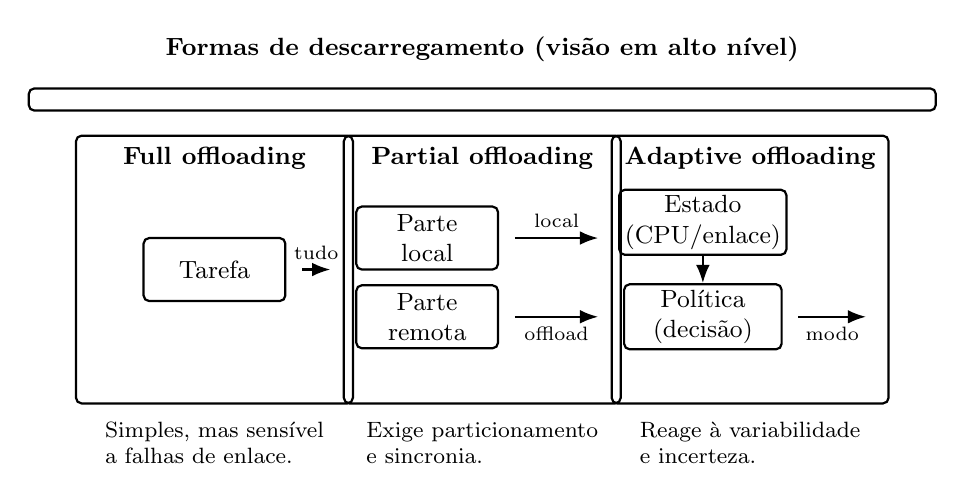
\begin{tikzpicture}[node distance=10mm]
  \node[vec/box, minimum width=0.95\linewidth] (frame) {};

  \node[vec/title, above=2mm of frame.north] {Formas de descarregamento (vis\~ao em alto n\'ivel)};

  % Colunas
  \node[vec/box, minimum width=0.29\linewidth, minimum height=34mm, anchor=north west] (full) at ($(frame.north west)+(6mm,-6mm)$) {};
  \node[vec/box, minimum width=0.29\linewidth, minimum height=34mm, anchor=north] (part) at ($(frame.north)+(0mm,-6mm)$) {};
  \node[vec/box, minimum width=0.29\linewidth, minimum height=34mm, anchor=north east] (adap) at ($(frame.north east)+(-6mm,-6mm)$) {};

  \node[vec/title] at ($(full.north)+(0mm,-3mm)$) {Full offloading};
  \node[vec/title] at ($(part.north)+(0mm,-3mm)$) {Partial offloading};
  \node[vec/title] at ($(adap.north)+(0mm,-3mm)$) {Adaptive offloading};

  % Full: bloco inteiro vai
  \node[vec/small, minimum width=18mm, minimum height=8mm] (tfull) at ($(full.center)+(0mm,0mm)$) {Tarefa};
  \draw[vec/arrow] ($(tfull.east)+(2mm,0)$) -- ($(full.east)+(-3mm,0)$) node[midway, above, font=\scriptsize] {tudo};

  % Partial: divide
  \node[vec/small, minimum width=18mm, minimum height=8mm] (tloc) at ($(part.center)+(-7mm,4mm)$) {Parte\\local};
  \node[vec/small, minimum width=18mm, minimum height=8mm] (toff) at ($(part.center)+(-7mm,-6mm)$) {Parte\\remota};
  \draw[vec/arrow] ($(tloc.east)+(2mm,0)$) -- ($(part.east)+(-3mm,4mm)$) node[midway, above, font=\scriptsize] {local};
  \draw[vec/arrow] ($(toff.east)+(2mm,0)$) -- ($(part.east)+(-3mm,-6mm)$) node[midway, below, font=\scriptsize] {offload};

  % Adaptive: chaveia com base no estado
  \node[vec/small, minimum width=20mm, minimum height=8mm] (state) at ($(adap.center)+(-6mm,6mm)$) {Estado\\(CPU/enlace)};
  \node[vec/small, minimum width=20mm, minimum height=8mm] (policy) at ($(adap.center)+(-6mm,-6mm)$) {Pol\'itica\\(decis\~ao)};
  \draw[vec/arrow] (state) -- (policy);
  \draw[vec/arrow] ($(policy.east)+(2mm,0)$) -- ($(adap.east)+(-3mm,-6mm)$) node[midway, below, font=\scriptsize] {modo};

  % Notas
  \node[vec/note, below=1mm of full.south] {Simples, mas sens\'ivel\\a falhas de enlace.};
  \node[vec/note, below=1mm of part.south] {Exige particionamento\\e sincronia.};
  \node[vec/note, below=1mm of adap.south] {Reage \`a variabilidade\\e incerteza.};

\end{tikzpicture}

\end{document}
